\documentclass[uplatex,dvipdfmx,11pt,fleqn]{jsarticle}

\usepackage{newtxtext}% 欧文フォント
\usepackage{newtxmath}% 数式フォント
\usepackage[
    dvipdfmx,hidelinks,
    pdftitle=ナノ結晶FeCoNiミディアムエントロピー合金の変形特性,
    pdfauthor=渡邉充哉 <watanabe@osakafu-u.net>
]{hyperref}
\usepackage{sotsuken}
\usepackage{booktabs}% 表組み
\usepackage{amsmath}
\usepackage[dvipdfmx]{graphicx}
\usepackage[uplatex,deluxe]{otf}% 多ウエイト対応

% フォントの設定
\DeclareFontShape{JY2}{hmc}{b}{n}{<->ssub*hmc/bx/n}{}
\DeclareFontShape{JT2}{hmc}{b}{n}{<->ssub*hmc/bx/n}{}
\DeclareFontShape{JT2}{hgt}{b}{n}{<->ssub*hgt/bx/n}{}
\DeclareFontShape{JY2}{hgt}{b}{n}{<->ssub*hgt/bx/n}{}

%\usepackage{color}
% \usepackage{mediabb}% xbbファイル読込み
% \usepackage{float}% 図H指定
%\setlength\intextsep{80zh}% 本文中の図の余白
\setlength\abovecaptionskip{0.5zh}% 図とキャプションとの余白
%\usepackage[subrefformat=parens]{subcaption}% サブキャプション
%\renewcommand{\thefootnote}{\fnsymbol{footnote}}% 脚注記号
\usepackage{pdfpages}
\usepackage[version=3]{mhchem}% 化学反応式
\usepackage{siunitx}% SI単位
% \sisetup{detect-all}
% \usepackage{multirow}% 段組み

% \usepackage{mathtools}\mathtoolsset{showonlyrefs=false}% 数式番号
\usepackage{empheq}% 連立方程式
%\allowdisplaybreaks[4]% 数式中の改ページ許可(0→4)

\usepackage{dcolumn}% 小数点揃え
%\usepackage{nidanfloat}% 図表段抜き
% \usepackage{balance}% 段ぞろえ
% \usepackage{wrapfig}% 図の回り込み
\usepackage[numbers,sort&compress]{natbib}

%titlepageここから
% \renewcommand{\title}{}%標題
% \renewcommand{\Engtitle}{}%英文標題
% \renewcommand{\reportnumber}{}%レポート番号
% \renewcommand{\thesis}{2021年度 修士論文}%レポート名
% \renewcommand{\edition}{}%レポートの種類・版表示
% \renewcommand{\id}{2200105128}%学籍番号
% \renewcommand{\author}{渡邉 充哉}%著者
% \renewcommand{\Engauthor}{Watanabe Atsuya}%英文著者名
% \renewcommand{\freespace}{}
% \renewcommand{\yearr}{2022}%発行年
% \renewcommand{\date}{2022年MM月DD日}%発行日
% \renewcommand{\editdata}{\date}
% \renewcommand{\organization}{大阪府立大学}
% \renewcommand{\department}{工学研究科 物質・化学系専攻 マテリアル工学分野}%発行者名
% \renewcommand{\Engdepartment}{Dept. Materials Science, Osaka Prefecture University}%英文発行者名
% \renewcommand{\address}{〒599-8531 大阪府堺市中区学園町1番1号}%発行者所在地
% \renewcommand{\tel}{xxx-xxxx-xxxx}%発行者電話番号
% \renewcommand{\mail}{watanabe@osakafu-u.net}

\begin{document}
%\maketitlepage% 表紙
\renewcommand{\thepage}{Title}% コレないとpdf上のページ番号がうまくいかない
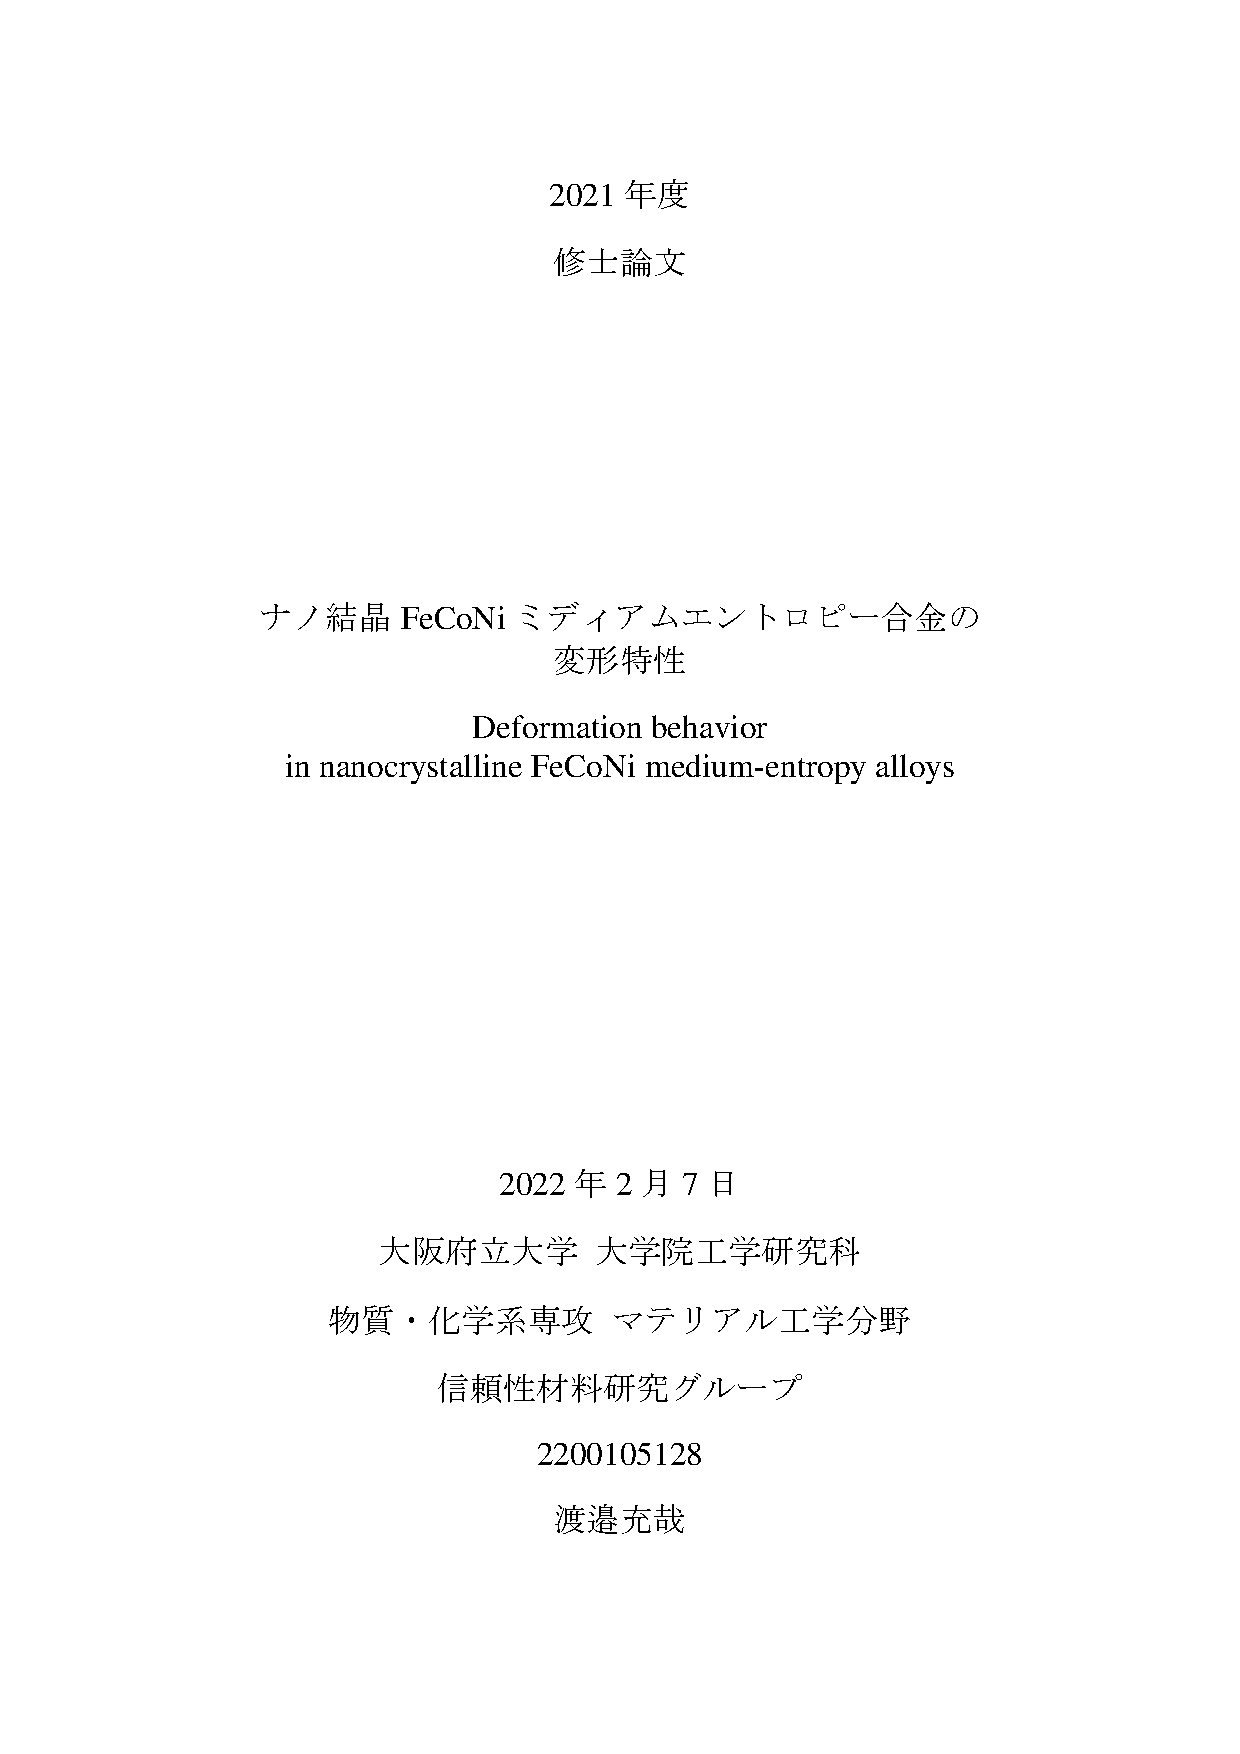
\includepdf{parts/frontpage.pdf}
\pagenumbering{roman}
% \makedocumentseet
\clearpage
\doublespacing
\section*{抄録 / Abstract}
\phantomsection
\addcontentsline{toc}{section}{抄録}
%#main ../watanabe_MasterThesis.tex

日本国民は、正当に選挙された国会における代表者を通じて行動し、われらとわれらの子孫のために、諸国民との協和による成果と、わが国全土にわたつて自由のもたらす恵沢を確保し、政府の行為によつて再び戦争の惨禍が起ることのないやうにすることを決意し、ここに主権が国民に存することを宣言し、この憲法を確定する。そもそも国政は、国民の厳粛な信託によるものであつて、その権威は国民に由来し、その権力は国民の代表者がこれを行使し、その福利は国民がこれを享受する。これは人類普遍の原理であり、この憲法は、かかる原理に基くものである。われらは、これに反する一切の憲法、法令及び詔勅を排除する。
日本国民は、恒久の平和を念願し、人間相互の関係を支配する崇高な理想を深く自覚するのであつて、平和を愛する諸国民の公正と信義に信頼して、われらの安全と生存を保持しようと決意した。われらは、平和を維持し、専制と隷従、圧迫と偏狭を地上から永遠に除去しようと努めてゐる国際社会において、名誉ある地位を占めたいと思ふ。われらは、全世界の国民が、ひとしく恐怖と欠乏から免かれ、平和のうちに生存する権利を有することを確認する。


We, the Japanese people, acting through our duly elected representatives in the National Diet, determined that we shall secure for ourselves and our posterity the fruits of peaceful cooperation with all nations and the blessings of liberty throughout this land, and resolved that never again shall we be visited with the horrors of war through the action of government, do proclaim that sovereign power resides with the people and do firmly establish this Constitution.Government is a sacred trust of the people, the authority for which is derived from the people, the powers of which are exercised by the representatives of the people, and the benefits of which are enjoyed by the people.This is a universal principle of mankind upon which this Constitution is founded.We reject and revoke all constitutions, laws, ordinances, and rescripts in conflict herewith.


\clearpage
\phantomsection
% \singlespacing
\addcontentsline{toc}{section}{目次}
\tableofcontents% 目次
%\thispagestyle{roman}% ページ番号消去
\clearpage
\pagenumbering{arabic}
\renewcommand{\thepage}{\arabic{page}}

% ==========記事ここから==========
\doublespacing
\section{緒言}
%#main ../watanabe_MasterThesis.tex

\subsection{天皇}
\subsubsection{社会的背景}
日本国民は、正当に選挙された国会における代表者を通じて行動し、われらとわれらの子孫のために、諸国民との協和による成果と、わが国全土にわたつて自由のもたらす恵沢を確保し、政府の行為によつて再び戦争の惨禍が起ることのないやうにすることを決意し、ここに主権が国民に存することを宣言し、この憲法を確定する。そもそも国政は、国民の厳粛な信託によるものであつて、その権威は国民に由来し、その権力は国民の代表者がこれを行使し、その福利は国民がこれを享受する。これは人類普遍の原理であり、この憲法は、かかる原理に基くものである。われらは、これに反する一切の憲法、法令及び詔勅を排除する。
日本国民は、恒久の平和を念願し、人間相互の関係を支配する崇高な理想を深く自覚するのであつて、平和を愛する諸国民の公正と信義に信頼して、われらの安全と生存を保持しようと決意した。われらは、平和を維持し、専制と隷従、圧迫と偏狭を地上から永遠に除去しようと努めてゐる国際社会において、名誉ある地位を占めたいと思ふ。われらは、全世界の国民が、ひとしく恐怖と欠乏から免かれ、平和のうちに生存する権利を有することを確認する。
われらは、いづれの国家も、自国のことのみに専念して他国を無視してはならないのであつて、政治道徳の法則は、普遍的なものであり、この法則に従ふことは、自国の主権を維持し、他国と対等関係に立たうとする各国の責務であると信ずる。
日本国民は、国家の名誉にかけ、全力をあげてこの崇高な理想と目的を達成することを誓ふ。

また,多結晶金属材料の強度は結晶粒径の$1/2$乗に反比例する(Hall-Petch則)。
したがって,結晶粒径の微細化により大幅な強度向上が期待できる~\cite{Watanabe2022}
\begin{align}
    H=H_0+d^{-1/2}
\end{align}

\subsubsection{金属材料の機械的特性}
日本国民は、正当に選挙された国会における代表者を通じて行動し、われらとわれらの子孫のために、諸国民との協和による成果と、わが国全土にわたつて自由のもたらす恵沢を確保し、政府の行為によつて再び戦争の惨禍が起ることのないやうにすることを決意し、ここに主権が国民に存することを宣言し、この憲法を確定する。そもそも国政は、国民の厳粛な信託によるものであつて、その権威は国民に由来し、その権力は国民の代表者がこれを行使し、その福利は国民がこれを享受する。これは人類普遍の原理であり、この憲法は、かかる原理に基くものである。われらは、これに反する一切の憲法、法令及び詔勅を排除する。
日本国民は、恒久の平和を念願し、人間相互の関係を支配する崇高な理想を深く自覚するのであつて、平和を愛する諸国民の公正と信義に信頼して、われらの安全と生存を保持しようと決意した。われらは、平和を維持し、専制と隷従、圧迫と偏狭を地上から永遠に除去しようと努めてゐる国際社会において、名誉ある地位を占めたいと思ふ。われらは、全世界の国民が、ひとしく恐怖と欠乏から免かれ、平和のうちに生存する権利を有することを確認する。
われらは、いづれの国家も、自国のことのみに専念して他国を無視してはならないのであつて、政治道徳の法則は、普遍的なものであり、この法則に従ふことは、自国の主権を維持し、他国と対等関係に立たうとする各国の責務であると信ずる。
日本国民は、国家の名誉にかけ、全力をあげてこの崇高な理想と目的を達成することを誓ふ。
\clearpage
\section{方法}
%#main ../watanabe_MasterThesis.tex

\subsection{合金元素の選択}
日本国民は、正当に選挙された国会における代表者を通じて行動し、われらとわれらの子孫のために、諸国民との協和による成果と、わが国全土にわたつて自由のもたらす恵沢を確保し、政府の行為によつて再び戦争の惨禍が起ることのないやうにすることを決意し、ここに主権が国民に存することを宣言し、この憲法を確定する。そもそも国政は、国民の厳粛な信託によるものであつて、その権威は国民に由来し、その権力は国民の代表者がこれを行使し、その福利は国民がこれを享受する。これは人類普遍の原理であり、この憲法は、かかる原理に基くものである。われらは、これに反する一切の憲法、法令及び詔勅を排除する。
日本国民は、恒久の平和を念願し、人間相互の関係を支配する崇高な理想を深く自覚するのであつて、平和を愛する諸国民の公正と信義に信頼して、われらの安全と生存を保持しようと決意した。われらは、平和を維持し、専制と隷従、圧迫と偏狭を地上から永遠に除去しようと努めてゐる国際社会において、名誉ある地位を占めたいと思ふ。われらは、全世界の国民が、ひとしく恐怖と欠乏から免かれ、平和のうちに生存する権利を有することを確認する。
われらは、いづれの国家も、自国のことのみに専念して他国を無視してはならないのであつて、政治道徳の法則は、普遍的なものであり、この法則に従ふことは、自国の主権を維持し、他国と対等関係に立たうとする各国の責務であると信ずる。
日本国民は、国家の名誉にかけ、全力をあげてこの崇高な理想と目的を達成することを誓ふ。

\clearpage
\section{結果と考察}
%#main ../watanabe_MasterThesis.tex

\subsection{Sample~A: bcc FeCoNi MEA}
\subsubsection{組織観察・組成分析}
日本国民は、正当に選挙された国会における代表者を通じて行動し、われらとわれらの子孫のために、諸国民との協和による成果と、わが国全土にわたつて自由のもたらす恵沢を確保し、政府の行為によつて再び戦争の惨禍が起ることのないやうにすることを決意し、ここに主権が国民に存することを宣言し、この憲法を確定する。そもそも国政は、国民の厳粛な信託によるものであつて、その権威は国民に由来し、その権力は国民の代表者がこれを行使し、その福利は国民がこれを享受する。これは人類普遍の原理であり、この憲法は、かかる原理に基くものである。われらは、これに反する一切の憲法、法令及び詔勅を排除する。
日本国民は、恒久の平和を念願し、人間相互の関係を支配する崇高な理想を深く自覚するのであつて、平和を愛する諸国民の公正と信義に信頼して、われらの安全と生存を保持しようと決意した。われらは、平和を維持し、専制と隷従、圧迫と偏狭を地上から永遠に除去しようと努めてゐる国際社会において、名誉ある地位を占めたいと思ふ。われらは、全世界の国民が、ひとしく恐怖と欠乏から免かれ、平和のうちに生存する権利を有することを確認する。

\begin{figure}
  \centering
  \includegraphics{example-image}
  \caption{電着FeCoNi合金のEDXスペクトル\label{fig:EDX}}
\end{figure}

\clearpage
\section{結言}
%#main ../watanabe_MasterThesis.tex

日本国民は、正当に選挙された国会における代表者を通じて行動し、われらとわれらの子孫のために、諸国民との協和による成果と、わが国全土にわたつて自由のもたらす恵沢を確保し、政府の行為によつて再び戦争の惨禍が起ることのないやうにすることを決意し、ここに主権が国民に存することを宣言し、この憲法を確定する。そもそも国政は、国民の厳粛な信託によるものであつて、その権威は国民に由来し、その権力は国民の代表者がこれを行使し、その福利は国民がこれを享受する。これは人類普遍の原理であり、この憲法は、かかる原理に基くものである。われらは、これに反する一切の憲法、法令及び詔勅を排除する。
日本国民は、恒久の平和を念願し、人間相互の関係を支配する崇高な理想を深く自覚するのであつて、平和を愛する諸国民の公正と信義に信頼して、われらの安全と生存を保持しようと決意した。われらは、平和を維持し、専制と隷従、圧迫と偏狭を地上から永遠に除去しようと努めてゐる国際社会において、名誉ある地位を占めたいと思ふ。われらは、全世界の国民が、ひとしく恐怖と欠乏から免かれ、平和のうちに生存する権利を有することを確認する。

% ==========記事ここまで==========

\clearpage
\phantomsection
\addcontentsline{toc}{section}{参照文献}
\bibliographystyle{Scripta-new-2}
\bibliography{parts/ref}

\clearpage
\phantomsection
\addcontentsline{toc}{section}{謝辞}
\section*{謝辞}
%#main ../watanabe_MasterThesis.tex

本研究は,著者が大阪府立大学大学院 工学研究科 博士前期課程在学中に
同研究科教授のとある先生の御指導のもと実施したものです。
研究の遂行にあたり,御指導を賜りましたこと,謹んで御礼申し上げます。

ここに感謝の意を表します。

\begin{flushright}
    2022-12-23 渡邉充哉
\end{flushright}

\clearpage

%\clearpage
%\clearpage
%\makeokuzuke
%\pagenumbering{roman}%
%\setcounter{page}{1}%
%\thispagestyle{empty}%
\end{document}